\documentclass{article}

\usepackage{fancyhdr}
\usepackage{extramarks}
\usepackage{amsmath}
\usepackage{amsthm}
\usepackage{amsfonts}
\usepackage{tikz}
\usepackage[plain]{algorithm}
\usepackage{algpseudocode}
\usepackage{enumitem}
\usepackage{pgfplots}
\usepackage{subcaption}

\usetikzlibrary{automata,positioning}

% Basic document settings
\topmargin=-0.45in
\evensidemargin=0in
\oddsidemargin=0in
\textwidth=6.5in
\textheight=9.0in
\headsep=0.25in

\linespread{1.1}

\pagestyle{fancy}
\lhead{\hmwkAuthorName}
\chead{\hmwkClass\ (\hmwkClassInstructor\ \hmwkClassTime): \hmwkTitle}
\rhead{\firstxmark}
\lfoot{\lastxmark}
\cfoot{\thepage}

\renewcommand\headrulewidth{0.4pt}
\renewcommand\footrulewidth{0.4pt}

\setlength\parindent{0pt}

% Pgfplots settings
\pgfplotsset{
    standard/.style={
        axis line style = thick,
        trig format=rad,
        enlargelimits,
        axis x line=middle,
        axis y line=middle,
        enlarge x limits=0.15,
        enlarge y limits=0.15,
        every axis x label/.style={at={(current axis.right of origin)}, anchor=north west},
        every axis y label/.style={at={(current axis.above origin)},anchor=south east},
        % grid=both,
        ticklabel style={font=\large, fill=white}
    }
}

% Create problem sections
\newcommand{\enterProblemHeader}[1]{
    \nobreak\extramarks{}{Problem \arabic{#1} continued on next page\ldots}\nobreak{}
    \nobreak\extramarks{Problem \arabic{#1}}{Problem \arabic{#1} continued on next page\ldots}\nobreak{}
}

\newcommand{\exitProblemHeader}[1]{
    \nobreak\extramarks{Problem \arabic{#1}}{Problem \arabic{#1} continued on next page\ldots}\nobreak{}
    \stepcounter{#1}
    \nobreak\extramarks{Problem \arabic{#1}}{}\nobreak{}
}

\setcounter{secnumdepth}{0}
\newcounter{partCounter}
\newcounter{homeworkProblemCounter}
\setcounter{homeworkProblemCounter}{1}
\nobreak\extramarks{Problem \arabic{homeworkProblemCounter}}{}\nobreak{}

% Homework problem environment
\newenvironment{homeworkProblem}[2][-1]{
    \ifnum#1>0
        \setcounter{homeworkProblemCounter}{#1}
    \fi
    \section{Problem \arabic{homeworkProblemCounter}: #2}
    \setcounter{partCounter}{1}
    \enterProblemHeader{homeworkProblemCounter}
}{
    \exitProblemHeader{homeworkProblemCounter}
}

% Homework details
\newcommand{\hmwkTitle}{Problem Set\ \#3}
\newcommand{\hmwkDueDate}{October 20, 2024}
\newcommand{\hmwkDueTime}{10:00pm}
\newcommand{\hmwkClass}{Macroeconomics}
\newcommand{\hmwkClassTime}{Section 104}
\newcommand{\hmwkClassInstructor}{Prof. Barnichon}
\newcommand{\hmwkAuthorName}{\textbf{Zachary Brandt}}

% Title page
\title{
    \vspace{2in}
    \textmd{\textbf{\hmwkClass:\ \hmwkTitle}}\\
    \normalsize\vspace{0.1in}\small{Due\ on\ \hmwkDueDate\ at \hmwkDueTime}\\
    \vspace{0.1in}\large{\textit{\hmwkClassInstructor\ \hmwkClassTime}}
    \vspace{3in}
}

\author{\hmwkAuthorName}
\date{}

% Various helper commands 

\renewcommand{\part}[1]{\textbf{\large Part \Alph{partCounter}}\stepcounter{partCounter}\\}

% Useful for algorithms
\newcommand{\alg}[1]{\textsc{\bfseries \footnotesize #1}}

% For derivatives
\newcommand{\deriv}[1]{\frac{\mathrm{d}}{\mathrm{d}x} (#1)}

% For partial derivatives
\newcommand{\pderiv}[2]{\frac{\partial}{\partial #1} (#2)}

% Integral dx
\newcommand{\dx}{\mathrm{d}x}

% Alias for the Solution section header
\newcommand{\solution}{\textbf{\large Solution}}

% Probability commands: Expectation, Variance, Covariance, Bias
\newcommand{\E}{\mathrm{E}}
\newcommand{\Var}{\mathrm{Var}}
\newcommand{\Cov}{\mathrm{Cov}}
\newcommand{\Bias}{\mathrm{Bias}}

\begin{document}

\maketitle

\pagebreak

\begin{homeworkProblem}[1]{Recovering from a War}
    Consider the basic Solow model with constant technology and constant 
    population. Recall that the key equations of this model are
    
    \begin{enumerate}[topsep=15pt]
        \item[(1)] \:\:\: $Y_t = \Bar{A}K_t^{1/3}\Bar{L}^{2/3}$
        \item[(2)] \:\:\: $I_t = \Bar{s}Y_t$
        \item[(3)] \:\:\: $C_t = Y_t-I_t$
        \item[(4)] \:\:\: $K_{t+1} = K_t+I_t-\Bar{d}K_t$
    \end{enumerate}
    
    A) Suppose the economy starts off with a capital stock $K_0$. Using the
    Solow diagram, explain how the capital stock will evolve over time.
    \\ \\
    B) Now starting from a point where none of the exogenous variables have 
    changed for a long period of time, suppose that a war occurs that destroys 
    a large part of the capital stock. Using time series plots (i.e., plots 
    with time on the x-axis and the variable being described on the y-axis), 
    describe the evolution of the capital stock and output due to the war 
    in qualitative terms. 
    \\ \\
    C) Recall that with competitive labor and capital markets the wage rate
    and the rental rate on capital will be given by
    \[
        \begin{split}
            \frac{2}{3}\Bar{A}\frac{K_t^{1/3}}{\Bar{L}^{1/3}} &= w_t
            \\
            \frac{1}{3}\Bar{A}\frac{\Bar{L}^{2/3}}{K_t^{2/3}} &= r_t
            \\
        \end{split}
    \]
    Using time series plots, describe the evolution of the wage rate and
    the rental rate on capital that occur due to the war in qualitative terms.

    \pagebreak
    \part
    
    Suppose the economy starts off with a capital stock $K_0$. Using the 
    Solow diagram, explain how the capital stock will evolve over time.
    \\ \\
    \solution
    \begin{center}
        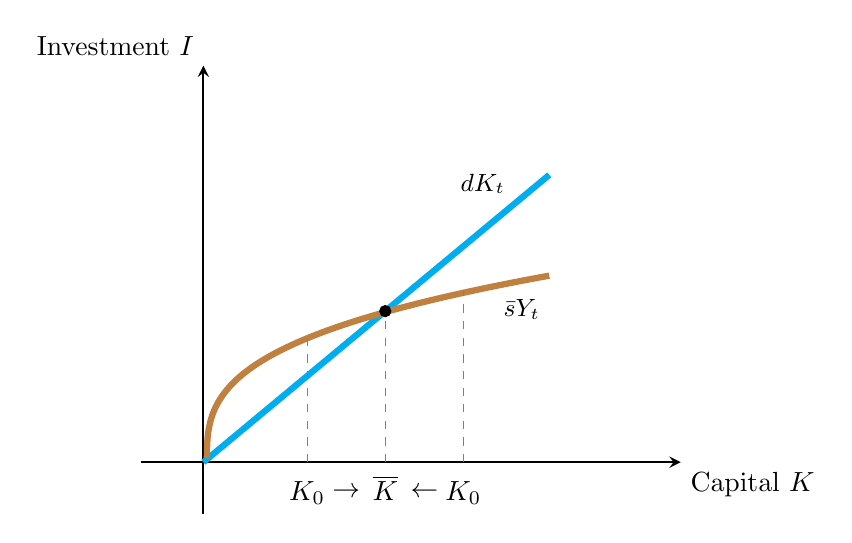
\begin{tikzpicture}
            \begin{axis}[standard,
                    ytick=\empty,
                    xtick=\empty,
                    xticklabels={},
                    yticklabels={},
                    xlabel={Capital $K$},
                    ylabel={Investment $I$},
                    samples=1000, 
                    xmin=0,
                    xmax=3,
                    ymin=0,
                    ymax=
                    3]
                \addplot[line width=0.8mm,cyan,domain={0:2.5}]{x};
                \addplot[line width=0.8mm,color=brown,domain={0:2.5}]{1.2*(x-0.025)^(1/3)};
                \addplot[mark=* , color=black] coordinates {(1.31453, 1.31453)}; 
                \addplot[dashed, gray, domain=0:1] coordinates {(1.31453,0) (1.31453,1.31453)};
                \node[anchor=center,label=south:{$\overline{K}$}] at (axis cs:1.31453,0.05){};
                \addplot[dashed, gray, domain=0:1] coordinates {(0.75,0) (0.75,1.09027)};
                \node[anchor=center,label=south:{$K_0$}] at (axis cs:0.75,0){};
                \addplot[dashed, gray, domain=0:1] coordinates {(1.879,0) (1.879,1.50)};
                \node[anchor=center,label=south:{$K_0$}] at (axis cs:1.879,0){};
                \node[anchor=center,label=south:{$\rightarrow$}] at (axis cs:1.032265,-0.05){};
                \node[anchor=center,label=south:{$\leftarrow$}] at (axis cs:1.597,-0.05){};
                \node[anchor=south east, color=black] at (axis cs:2.25, 2.25) {\small $dK_t$};
                \node[anchor=north west, color=black] at (axis cs:2.1, 1.5) {\small $\Bar{s}Y_t$};
            \end{axis}
        \end{tikzpicture} 
    \end{center}

    No matter the initial starting conditions of the economy, the capital 
    stock will increase or decrease over time to reach steady state. Steady 
    state is where the investment in capital $\overline{s}Y_t$ is equal 
    to the depreciation of capital $\overline{d}K_t$. At this point the 
    capital stock will remain constant over time. The above Solow diagram 
    shows the direction in which the capital stock will move from $K_0$.
    \\ \\
    At steady state $K_{t+1} = K_t = \overline{K}$ and we can use our equations
    to substitute and solve for $\overline{K}$
    \[
        \begin{split}
            \overline{K} &= \overline{K}+I_t-\overline{dK}
            \\
            \text{from (2)} \;\;\; \overline{dK} &= \overline{s}\overline{Y}
            \\
            \text{from (1)} \;\;\; \overline{dK} &= \overline{s}\overline{A}\overline{K}^{1/3}\overline{L}^{2/3}
            \\
            \overline{K}^{2/3} &= \frac{\overline{s}\overline{A}}{\overline{d}}\overline{L}^{2/3}
            \\
            \overline{K} &= \left( \frac{\overline{s}\overline{A}}{\overline{d}} \right)^{3/2}\overline{L}
        \end{split}
    \]
    The above result confirms that the steady state value of $K$ does not
    depend on the initial conditions but only on our exogenous model 
    parameters.

    \pagebreak
    \part

    Now starting from a point where none of the exogenous variables have 
    changed for a long period of time, suppose that a war occurs that destroys 
    a large part of the capital stock. Using time series plots (i.e., plots 
    with time on the x-axis and the variable being described on the y-axis), 
    describe the evolution of the capital stock and output due to the war
    in qualitative terms. 
    \\ \\
    \solution 
    \\
    If none of the exogenous variables have changed for a long period of 
    time, then output and capital will have reached their steady state
    values of $\overline{Y}$ and $\overline{K}$ respectively. Due to the
    war that destroys a large part of the capital stock, output and 
    capital will fall briefly to $Y_0$ and $K_0$ respectively. Over time,
    if none of the model parameters have changed, the economy will recover
    and output and capital will return to their steady state values.
    \\ \\
    % To find these time series plots of $Y_t$ and $K_t$ we need to solve the
    % differential equation $\frac{dK}{dt} = sAK^{1/3}L^{2/3} - dK$ from (4). 
    % General  solutions to this nonlinear differential equation take the form
    % \[
    %     \begin{split}
    %         K_t = \overline{K} - \left( K_0 - \overline{K} \right)e^{-dt}
    %     \end{split}
    % \]
    % and subsituting in our expression for $\overline{K}$ our time series 
    % plots for output and capital are
    % \[
    %     \begin{split}
    %         K_t &= \left( \frac{\overline{s}\overline{A}}{\overline{d}} \right)^{3/2}\overline{L} - \left( K_0 - \left( \frac{\overline{s}\overline{A}}{\overline{d}} \right)^{3/2}\overline{L} \right)e^{-dt}
    %         \\
    %         Y_t &= \overline{A} K_t^{1/3} \overline{L}^{2/3} \;\;\; \text{from (1)}
    %     \end{split}
    % \]
    Two potential time series plots for $Y_t$ and $K_t$ are shown below. The 
    first plot is of $K_t$ and the second plot is of $Y_t$. While the exact shape 
    of these plots will depend on the initial conditions and the model parameters,
    the general shape of the recovery should look the same as below.
    \\ \\
    \begin{minipage}{0.5\textwidth}
        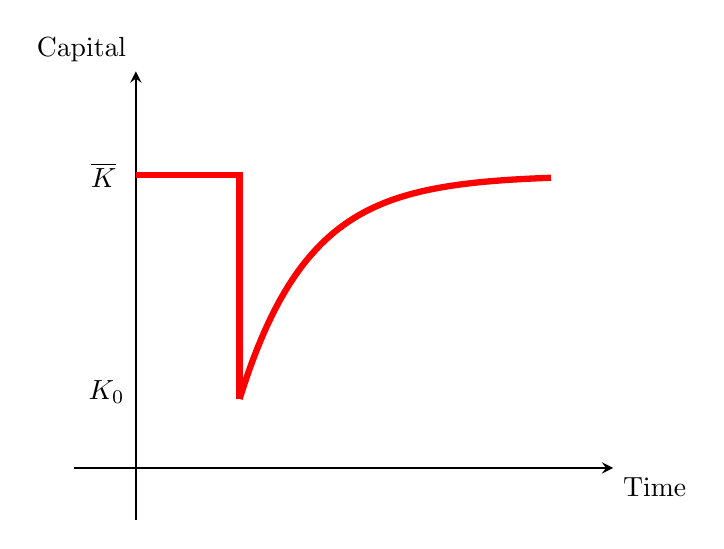
\begin{tikzpicture}
            \begin{axis}[standard,
                    ytick=\empty,
                    xtick=\empty,
                    xticklabels={},
                    yticklabels={},
                    xlabel={Time},
                    ylabel={Capital},
                    samples=1000, 
                    xmin=0,
                    xmax=20,
                    ymin=0,
                    ymax=5]
                \addplot[line width=0.8mm,red,domain={0:5}]{4.243};
                \addplot[line width=0.8mm,red,domain={5:20}]{4.243+(1-4.243)*exp(-0.3*(x-5))};
                \addplot[line width=0.8mm,red,domain=0:5] coordinates {(5,1) (5,4.29)};
                \node[anchor=center,label=west:{$\overline{K}$}] at (axis cs:0,4.243){};
                \node[anchor=center,label=west:{$K_0$}] at (axis cs:0.4,1.1){};
            \end{axis}
        \end{tikzpicture}    
    \end{minipage}
    \begin{minipage}{0.5\textwidth}
        \begin{tikzpicture}
                \begin{axis}[standard,
                        ytick=\empty,
                        xtick=\empty,
                        xticklabels={},
                        yticklabels={},
                        xlabel={Time},
                        ylabel={Output},
                        samples=1000, 
                        xmin=0,
                        xmax=20,
                        ymin=0,
                        ymax=4]
                    \addplot[line width=0.8mm,red,domain={0:5}]{3.182};
                    \addplot[line width=0.8mm,red,domain={5:20}]{1.966*(4.243+(1-4.243)*exp(-0.3*(x-5)))^(1/3)};
                    \addplot[line width=0.8mm,red,domain=0:5] coordinates {(5,1.966) (5,3.22)};
                    \node[anchor=center,label=west:{$\overline{Y}$}] at (axis cs:0,3.182){};
                    \node[anchor=center,label=west:{$Y_0$}] at (axis cs:0.4,1.966){};
                \end{axis}
            \end{tikzpicture}    
    \end{minipage}
    \\ \\ \\
    From the above, we can see that the capital stock and output fall sharply
    to $K_0$ and $Y_0$ respectively due to the war. Over time, the economy 
    will recover and both capital and output will approach their steady 
    states as time goes to infinity.
    \\ \\
    The recovery in the capital stock and output, which is a function of the capital
    stock, share a similar pattern: initially a very sharp recovery that levels
    off. Considering equation (4) from the problem specification, this makes sense
    since investment $I_s$ will initially be far greater than the depreciation
    $\overline{d}K_t$ since $K$ has fallen so dramatically and because the cube
    root function of capital in output (which determines $I_s$) initally grows
    quickly. However, as we approach steady state, the two will get closer to
    cancelling as there are diminishing returns to output from additional capital
    and because depreciation grows directly with the capital stock.
    

    \pagebreak
    \part

    Recall that with competitive labor and capital markets the wage rate 
    and the rental rate on capital will be given by
    \[
        \begin{split}
            \frac{2}{3}\Bar{A}\frac{K_t^{1/3}}{\Bar{L}^{1/3}} &= w_t
            \\
            \frac{1}{3}\Bar{A}\frac{\Bar{L}^{2/3}}{K_t^{2/3}} &= r_t
            \\
        \end{split}
    \]
    Using time series plots, describe the evolution of the wage rate and 
    the rental rate on capital that occur due to the war in qualitative terms.
    \\ \\
    \solution
    \\
    First we need to find the long run equilibrium wage rate and rental rate 
    on capital. Substituting our expression for $\overline{K}$ into the above 
    equations for $w_t$ and $r_t$ we get
    \[
        \begin{split}
            \overline{w} &= \frac{2}{3}\Bar{A}\frac{\left( \left( \frac{\overline{s}\overline{A}}{\overline{d}} \right)^{3/2}\overline{L} \right)^{1/3}}{\Bar{L}^{1/3}} = \frac{2}{3}\Bar{A}\left( \frac{\overline{s}\overline{A}}{\overline{d}} \right)^{1/2}
            \\ \\ 
            \overline{r} &= \frac{1}{3}\Bar{A}\frac{\Bar{L}^{2/3}}{\left( \left( \frac{\overline{s}\overline{A}}{\overline{d}} \right)^{3/2}\overline{L} \right)^{2/3}} = \frac{1}{3}\Bar{A}\left( \frac{\overline{d}}{\overline{s}\overline{A}} \right)
        \end{split}
    \]

    We can create the time series plots for the wage rate and the rental 
    rate on capital by substituting in a time series expression for 
    $K_t$ from B) into the equations for $w_t$ and $r_t$ and plotting.
    Two possible plots for the wage rate and rental rate on capital 
    respectively are shown below.
    \\ \\
    \begin{minipage}{0.5\textwidth}
        \begin{tikzpicture}
            \begin{axis}[standard,
                    ytick=\empty,
                    xtick=\empty,
                    xticklabels={},
                    yticklabels={},
                    xlabel={Time},
                    ylabel={Wage},
                    samples=1000, 
                    xmin=0,
                    xmax=20,
                    ymin=0,
                    ymax=2]
                \addplot[line width=0.8mm,red,domain={0:5}]{1.414};
                \addplot[line width=0.8mm,red,domain={5:20}]{(0.874)*(4.243+(-3.243)*exp(-0.3*(x-5)))^(1/3)};
                \addplot[line width=0.8mm,red,domain=0:5] coordinates {(5,0.875) (5,1.424)};
                \node[anchor=center,label=west:{$\overline{w}$}] at (axis cs:0,1.414){};
                \node[anchor=center,label=west:{$w_0$}] at (axis cs:0.4,0.875){};
            \end{axis}
        \end{tikzpicture}
    \end{minipage}
    \begin{minipage}{0.5\textwidth}   
        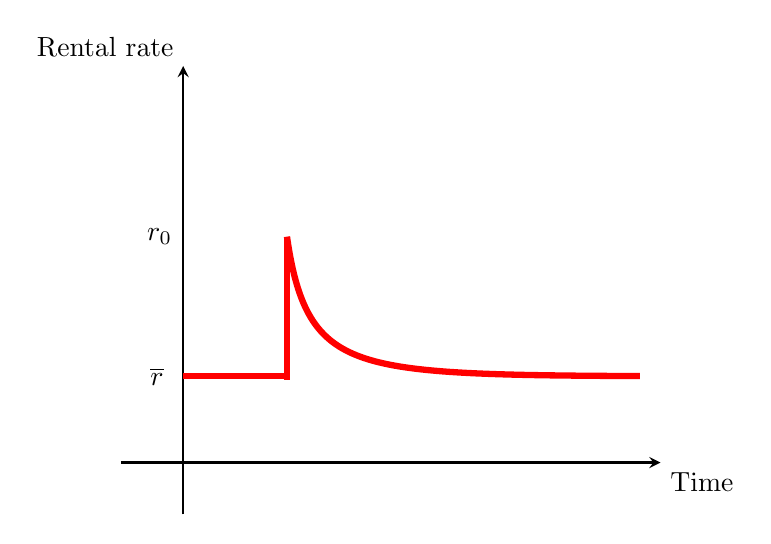
\begin{tikzpicture}
            \begin{axis}[standard,
                    ytick=\empty,
                    xtick=\empty,
                    xticklabels={},
                    yticklabels={},
                    xlabel={Time},
                    ylabel={Rental rate},
                    samples=1000, 
                    xmin=0,
                    xmax=20,
                    ymin=0,
                    ymax=1]
                \addplot[line width=0.8mm,red,domain={0:5}]{0.25};
                \addplot[line width=0.8mm,red,domain={5:22}]{(0.655)*(4.243+(-3.243)*exp(-0.3*(x-5)))^(-2/3)};
                \addplot[line width=0.8mm,red,domain=0:5] coordinates {(5,0.24) (5,0.655)};
                \node[anchor=center,label=west:{$\overline{r}$}] at (axis cs:0,0.25){};
                \node[anchor=center,label=west:{$r_0$}] at (axis cs:0.4,0.655){};
            \end{axis}
        \end{tikzpicture}
    \end{minipage}
    \\ \\ \\
    From the above plots we can see that the wage rate will fall sharply to 
    $w_0$ and the rental rate will spike to $r_0$ respectively due to the war.
    This makes sense considering the expressions for the marginal products of 
    labor and capital in this problem specification, which equal $w_t$ and $r_t$
    respectively. In the case of the wage, $w_t \propto K_t^{1/3}$, whereas
    for the rental rate, $r_t \propto K_t^{-2/3}$. That is, the wage rate will
    fall with the capital stock, as workers' product decreases, while the rental
    rate will shoot up as $r_t$ is decreasing in $K$, which makes sense considering
    supply-and-demand mechanics.

\end{homeworkProblem}

\pagebreak

\begin{homeworkProblem}[2]{Misallocation and TFP}
    One lesson from the Solow model is that the determinants of long-run 
    growth have to be found in total factor productivity $A_t$. Since $A_t$
    is measured as the residual of a growth accounting decomposition, TFP
     is often referred to as a measure of our ignorance. 
    \\ \\
    A recent insight from the academic literature on economic growth is that 
    TFP can be affected by the allocation of factor inputs. This excercise 
    will introduce you to this idea. 
    \\ \\
    Suppose output is produced using two tasks according to $Y=X_1^{\alpha}X_2^{1-\alpha}$. 
    The tasks could be management vs. production work, manufacturing vs. 
    services, or private sector work vs. public (e.g., regulatory, judicial, 
    police) work. 
    \\ \\
    One unit of labor can produce one unit of either task, and the economy 
    is endowed with $L$ units of labor. Finally, suppose that the allocation 
    of labor is such that a fraction $s$ of total labor works in the first 
    task, and the fraction $1-s$ works in the second task. 
    \\ \\
    A) Derive a production function of the form $Y=f(L)$, and derive an 
    expression for TFP of this production function. 
    \\ \\
    B) Draw how TFP depends on the task allocation $s$ (recall $s \in [0,1])$.
    \\ \\
    C) What is the output maximizing allocation $s^*$? What happens to TFP then?
    \\ \\
    D) In many developing countries, taxes, poor management, information 
    problems, or corruption can lead to a non-optimal allocation of tasks.
    How can this 'theory explain that some countries remain poorer than 
    the US? 

    \pagebreak
    \part

    Derive a production function of the form $Y=f(L)$, and derive an expression 
    for TFP of this production function. 
    \\ \\
    \solution
    \\
    A production function of the form $Y=f(L)$ given in the problem specification 
    could be the following
    \[
        \begin{split}
            Y &= (sL)^{\alpha}((1-s)L)^{1-\alpha}
            \\
            Y &= s^{\alpha}(1-s)^{1-\alpha}L
        \end{split}
    \]
    The production function is broken into two tasks, $X_1$ and $X_2$, where
    $X_1$ is the task that requires $s$ units of labor and $X_2$ is the task
    that requires $(1-s)$ units of labor. The total output $Y$ is the product
    of the output of each task.
    \\ \\
    Total Factor Productivity is the ratio of output to input, or that portion
    of growth not explained by the change in inputs. In our case, we can 
    divide output by the change in the labor input to find TFP.
    \[
        A = \frac{Y}{L} = s^{\alpha}(1-s)^{1-\alpha}
    \]
    
    \pagebreak
    \part

    Draw how TFP depends on the task allocation $s$ (recall $s \in [0,1])$.
    \\ \\
    
    \solution
    \\
    Below I have plotted three different TFP functions for different values
    of $\alpha$. The first plot is for $\alpha = 0.25$, the second plot is
    for $\alpha = 0.5$, and the third plot is for $\alpha = 0.75$. The
    general shape of the TFP function is a bell curve with a maximum at
    $s = \alpha$.
    \\
    \begin{figure}[h!]
        \centering
        \begin{subfigure}{0.3\textwidth}
            \centering
            \begin{tikzpicture}
                \begin{axis}[
                    width=\textwidth,
                    height=0.8\textwidth,
                    xlabel={$s$},
                    ylabel={},
                    domain=0:1,
                    samples=100,
                    ymin=0, ymax=1,
                    axis lines=middle,
                    xtick={\empty},
                    ytick={\empty},
                    title={$ \alpha = 0.25 $},
                    xlabel style={at={(axis description cs:1,-0.1)}, anchor=north},]
                    \addplot[red, thick] {x^0.25*(1-x)^0.75};
                \end{axis}
            \end{tikzpicture}
        \end{subfigure}
        \begin{subfigure}{0.3\textwidth}
            \centering
            \begin{tikzpicture}
                \begin{axis}[
                    width=\textwidth,
                    height=0.8\textwidth,
                    xlabel={$s$},
                    domain=0:1,
                    samples=100,
                    ymin=0, ymax=1,
                    axis lines=middle,
                    xtick={\empty},
                    ytick={\empty},
                    title={$ \alpha = 0.5 $},
                    xlabel style={at={(axis description cs:1,-0.1)}, anchor=north},]
                    \addplot[red, thick] {x^0.5*(1-x)^0.5};
                \end{axis}
            \end{tikzpicture}
        \end{subfigure}
        \begin{subfigure}{0.3\textwidth}
            \centering
            \begin{tikzpicture}
                \begin{axis}[
                    width=\textwidth,
                    height=0.8\textwidth,
                    xlabel={$s$},
                    domain=0:1,
                    samples=100,
                    ymin=0, ymax=1,
                    axis lines=middle,
                    xtick={\empty},
                    ytick={\empty},
                    title={$ \alpha = 0.75 $},
                    xlabel style={at={(axis description cs:1,-0.1)}, anchor=north},]
                    \addplot[red, thick] {x^0.75*(1-x)^0.25};
                \end{axis}
            \end{tikzpicture}
        \end{subfigure}
    \end{figure}
    \\
    From the above plots we can see that TFP is maximized at some value of $s$
    between 0 and 1. The exact value of $s$ that maximizes TFP is $\alpha$,
    which is shown in the next part.

    \pagebreak
    \part

    What is the output maximizing allocation $s^*$? What happens to TFP then?
    \\ \\
    \solution
    \\
    Output in this case is maximized when TFP is maximized. We can find the
    optimal allocation $s^*$ by taking the derivative of TFP with respect 
    to a change in $s$ and setting the result equal to zero
    \[
        \begin{split}
            \frac{dA}{ds} &= \frac{d}{ds}\left( s^\alpha(1-s)^{1-\alpha} \right)
            \\
            &= \alpha s^{\alpha-1}(1-s)^{1-\alpha} - s^{\alpha}(1-\alpha)(1-s)^{-\alpha}   
            \\
            0 &= \alpha s^{\alpha-1}(1-s)^{1-\alpha} - s^{\alpha}(1-\alpha)(1-s)^{-\alpha}   
            \\
            s^{\alpha}(\alpha-1)(1-s)^{-\alpha} &= \alpha s^{\alpha-1}(1-s)^{1-\alpha}
            \\
            s^{\alpha}(1-\alpha) &= \alpha s^{\alpha-1}(1-s)
            \\
            s(1-\alpha) &= \alpha (1-s)
            \\
            s-s\alpha &= \alpha - \alpha s
            \\
            s &= \alpha
        \end{split}
    \]

    From this we can see the optimal allocation $s^*$ is reached when 
    $s = \alpha$. At this point, TFP is maximized and the economy is
    producing output at its maximum level given a fixed amount of labor.

    \pagebreak
    \part

    In many developing countries, taxes, poor management, information problems, 
    or corruption can lead to a non-optimal allocation of tasks. How can 
    this theory explain that some countries remain poorer than the US?
    \\ \\
    \solution
    \\
    If in these developing countries there are factors that prohibit an efficient
    task allocation $s$, then TFP will be lower than it could be. Considering that
    under the Solow model there is only long run per capita growth with increasing
    TFP, these countries will remain poorer than the US and not converge to the 
    same level of output and output per capita if their allocation of labor remains
    inefficient.
    
    
        
\end{homeworkProblem}

\pagebreak

\begin{homeworkProblem}[3]{From Land to Fossil Energy}
    Consider the Malthus model of population growth with $\frac{N_{t+1}}{N_t} = (\frac{w_t}{w_s})$.
    \\ \\
    In the model we saw in class, we had the production function $Y_t = D^{\alpha}N_t^{1-\alpha}$, where land $D$ was fixed. In that economy, wages are stuck at subsistence levels in the long-run.
    \\ \\
    But imagine that we discover abundant (underground) fossil fuels so that land is only needed for food, making the land constraint effectively no longer binding so that we can assume that there is always enough land to grow in line with population. Instead, energy becomes a central part of the production process, and the function becomes the function $Y_t=E_t^{\gamma}L_{y,t}^{1-\gamma}$ with $\gamma < 1$ and $L_{y,t}$ is labor employed in the production of final goods $Y$.
    \\ \\
    Extracting energy from the ground requires labor and the production process for energy is $E_t=L_{e,t}$ with $L_{e,t} = sN_t$, where the fraction of the population devoted to energy extraction ($s$) is fixed. The rest of the population is devoted to production of $Y_t$, so $L_{y,t}=(1-s)N_t$.
    \\ \\
    It will be useful to define the term $g = (1-\gamma)(\frac{s}{1-s})^{\gamma}/w_s$. We assume that $g>1$.
    \\ \\
    A) Derive the equation for the wage rate $w_t$ in the final goods sector. Given the Malthus population dynamics $\frac{N_{t+1}}{N_t} = (\frac{w_t}{w_s})$, what is the population growth rate?
    \\ \\
    B) What is the economy's growth rate (i.e., the growth rate of $Y_t$)? What is the per capita growth rate (i.e., the growth rate of $Y_t/N_t$)?
    \\ \\
    C) How do workers fare in this economy compared to (i) a Malthusian economy, and (ii) a Solow economy (with constant $A_t$) that we saw in class?
    \\ \\
    D) Derive the level of energy extracted at each date $t$, i.e., derive an expression for $E_t$ as a function of initial conditions $N_0$ (the population at date 0). Derive the \textit{total} amount of energy extracted since time 0.
    \\ \\
    E) Fossil energy is in fact in finite supply on Earth. At which date $\tau$ will we have exhausted all fossil fuel? Derive an expression for $\tau$ as a function of model paramters. What will happen then to growth?

    \pagebreak
    \part

    Derive the equation for the wage rate $w_t$ in the final goods sector. Given the Malthus population dynamics $\frac{N_{t+1}}{N_t} = (\frac{w_t}{w_s})$, what is the population growth rate?
    \\ \\
    \solution
    \\
    To find the wage rate $w_t$ for labor employed in the final goods sector, we find the marginal product of labor in the production fo these final goods by taking the partial derivative of output with respect to a change in $L_{y,t}$
    \[
        \begin{split}
            w_t = \frac{\partial Y_t}{\partial L_{y,t}} &= \frac{\partial}{\partial L_{y,t}} \left( E_t^{\gamma}L_{y,t}^{1-\gamma} \right)
            \\
            &= (1-\gamma)L_{e,t}^{\gamma}L_{y,t}^{-\gamma}
            \\
            &= (1-\gamma)\frac{s^{\gamma}N_t^{\gamma}}{(1-s)^{\gamma}N_t^{\gamma}}
            \\
            &= (1-\gamma)\left( \frac{s}{1-s} \right)^\gamma
        \end{split}
    \]

    Given this expression for our $w_t$, we can find the population growth rate by subsitution
    \[
        \begin{split}
            \frac{N_{t+1}}{N_t} &= \left( \frac{w_t}{w_s} \right)
            \\
            \frac{N_{t+1}}{N_t} &= \frac{(1-\gamma)\left( \frac{s}{1-s} \right)^{\gamma}}{w_s}
            \\
            \frac{N_{t+1}}{N_t} &= g
        \end{split}
    \]

    So our population growth rate in this economy becomes our term $g$ defined earler in the problem specification. The population as a function of time $t$ is then $N_t = N_0 g^t$ since
    \[
        \begin{split}
            N_{t+1} &= N_tg
            \\
            t=0 \;\;\;\; N_1 &= N_0g
            \\
            t=1 \;\;\;\; N_2 &= N_1g = N_0 g^2
            \\
            t=2 \;\;\;\; N_3 &= N_2g=N_0 g^3
            \\
            &\dots
            \\
            N_t &= N_0 g^t
        \end{split}
    \]

    \pagebreak
    \part

    What is the economy's growth rate (i.e., the growth rate of $Y_t$)? What is the per capita growth rate (i.e., the growth rate of $Y_t/N_t$)?
    \\ \\
    \solution
    \\
    To find the economy's growth rate, we find the change in output with respect to a change in time using the first time derivative of $Y_t$. First, I will simplify the expression for output so that it is only in terms of $s$, $\gamma$, and $N_t$

    \[
        \begin{split}
            Y_t &= E_t^{\gamma}L_{y,t}^{1-\gamma}
            \\
            &= L_{e,t}^{\gamma}L_{y,t}^{1-\gamma}
            \\
            &= (sN_t)^{\gamma}((1-s)N_t)^{1-\gamma}
            \\
            &= s^{\gamma}(1-s)^{1-\gamma}N_t
        \end{split}
    \]

    Now to find the growth rate I'll take the ratio of two consecutive time periods for output
    \[
        \begin{split}
            \frac{Y_{t+1}}{Y_t} &= \frac{s^{\gamma}(1-s)^{1-\gamma}N_{t+1}}{s^{\gamma}(1-s)^{1-\gamma}N_{t}}
            \\
            &= \frac{N_{t+1}}{N_t}
            \\
            &= g
        \end{split}
    \]
    From the above expression we can see that the economy's growth rate is equal to the population growth rate, $g$. To find the per capita growth rate, I'll divide the expression for output growth $Y_t$ by population growth $N_t$
    \[
        \begin{split}
            \frac{Y_{t+1}/Y_t}{N_{t+1}/N_t} &= \frac{Y_{t+1}}{Y_t} \cdot \frac{N_t}{N_{t+1}}
            \\
            &= g \cdot \frac{1}{g}
            \\
            &= 1
        \end{split}
    \]
    From the above, we can see that output growth with respect to population growth 
    is constant, so there is no per capita growth in output over time under this model.
    
    \pagebreak
    \part

    How do workers fare in this economy compared to (i) a Malthusian economy, and (ii) a Solow economy (with constant $A_t$) that we saw in class?
    \\ \\
    \solution
    \\
    Compared to a Malthusian econonmy, wages don't fall off with population
    growth. Instead, wages are fixed at a level determined by the fraction
    of the population devoted to energy extraction and the fraction of the
    population devoted to final goods production. In a Malthusian economy,
    any wage growth is offset in the long run by population growth which
    pushes them back down.
    \\ \\
    Compared to a Solow economy with a constant $A_t$, i.e, constant TFP,
    there is also no long run growth in output per capita. In the Solow
    model, only growth in TFP over time can lead to long run growth in
    output per capita. In this economy, output growth is similarly 
    determined only by population growth, and dividing by population
    simply cancels out the population growth term, rendering per capita
    output constant over time.


    \pagebreak
    \part

    Derive the level of energy extracted at each date $t$, i.e., derive an expression for $E_t$ as a function of initial conditions $N_0$ (the population at date 0). Derive the \textit{total} amount of energy extracted since time 0.
    \\ \\
    \solution
    \\
    To derive the level of energy extracted $E_t$ as a function of initial conditions $N_0$, we can substitute in our expression for $N_t$ in terms of $N_0$, $g$, and $t$
    \[
        \begin{split}
            E_t = L_{e,t} = sN_t = sN_0g^t
        \end{split}
    \]
    To derive the total amount of energy extracted since $t=0$, we can perform an integral to sum all the infinitesimal changes in energy with respect to a change in time
    \[
        \begin{split}
            \int_0^t E_t \, dt &= \int_0^t sN_0g^t \, dt
            \\
            &= sN_0 \int_0^t e^{tln(g)} \, dt
            \\
            &= \frac{sN_0}{ln(g)} \left( e^{tln(g)} - 1 \right)
            \\
            &= \frac{sN_0}{ln(g)} \left( g^t - 1 \right)
        \end{split}
    \]

    \pagebreak
    \part

    Fossil energy is in fact in finite supply on Earth. At which date $\tau$ will we have exhausted all fossil fuel? Derive an expression for $\tau$ as a function of model paramters. What will happen then to growth?
    \\ \\ 
    \solution
    \\
    We can find the time $\tau$ when all fossil fuels reserves have been exhausted when $\int_0^\tau E_t \, dt$ is equal to some $E_{\text{total}}$, which encapsulates the Earth's fossil fuel reserves.
    \[
        \begin{split}
            E_\text{total} &= \int_0^\tau E_t \, dt
            \\
            E_\text{total} &= \frac{sN_0}{ln(g)} \left( g^\tau - 1 \right)
            \\
            \frac{ln(g)}{sN_0} E_\text{total} &= g^\tau - 1
            \\
            g^\tau &= \frac{ln(g)}{sN_0} E_\text{total} + 1
            \\
            \tau ln(g) &= ln \left( \frac{ln(g)}{sN_0} E_\text{total} + 1 \right)
            \\
            \tau &= \frac{ln \left( \frac{ln(g)}{sN_0} E_\text{total} + 1 \right)}{ln(g)}
        \end{split}
    \]
    For times where $t>\tau$, output will be drastically decreased as $E_t = 0$ and should revert back to our Malthusian production model where land once again becomes a binding constraint on output.
\end{homeworkProblem}

\end{document}
